% !TEX program = pdflatex
% Homework template

\documentclass[12pt,en]{homework}
% en is for English language
% cn is for Chinese language

%----- text fonts -----
%\usepackage{newtxtext}
%\setmainfont{Times New Roman}

%----- math font -----
%\usepackage{newtxmath}
%\usepackage{mathptmx}
%\usepackage{mathpazo}

% custom theorem
\newtheorem{innercustomgeneric}{\customgenericname}
\providecommand{\customgenericname}{}
\newcommand{\newcustomtheorem}[2]{%
  \newenvironment{#1}[1]
  {%
   \renewcommand\customgenericname{#2}%
   \renewcommand\theinnercustomgeneric{##1}%
   \innercustomgeneric
  }
  {\endinnercustomgeneric}
}

\newcustomtheorem{ntheorem}{Theorem}
\newcustomtheorem{nlemma}{Lemma}

% differential operator
\newcommand{\dif}{\mathop{}\!\mathrm{d}}

% new command
\newcommand{\CC}{\ensuremath{\mathbb{C}}}
\newcommand{\RR}{\ensuremath{\mathbb{R}}}
\newcommand{\A}{\mathcal{A}}
\newcommand{\bA}{\boldsymbol{A}}
\newcommand{\ii}{\mathrm{i}\,}
\newcommand{\dx}[1][x]{\mathop{}\!\mathrm{d}#1}
\newcommand{\abs}[1]{\lvert#1\rvert}
\newcommand{\norm}[1]{\left\lVert#1\right\rVert}
\newcommand{\red}[1]{\textcolor{red}{#1}}

%------------------------------------------------------------
%	ASSIGNMENT INFORMATION
%------------------------------------------------------------

\header{Numerical methods of differential equation: Assignment \#1} % Header

\title{Assignment \#1} % Assignment

\author{Student name} % Student name

\date{\today} % Date
%\date{April 2, 2023}

\institute{Institute or school name} % Institute or school name

\courseinfo{Course: Numerical methods of differential equation} % Course info

\studentinfo{Major: XXX \quad Student ID: 123002584} % Student info


\begin{document}

\maketitle

%------------------------------------------------------------
%	ASSIGNMENT CONTENT
%------------------------------------------------------------

%\section*{Problem}

%------------------------------%

\begin{problem}
Here is a question.
\end{problem}

\begin{solution}
Here is the answer of the question.
\end{solution}

%------------------------------%

\begin{problem}
Here is a proof question.
\end{problem}

\begin{proof}
Here is the proof of the problem.
\end{proof}

%------------------------------%

\vspace{3em}

\begin{definition}\label{def:foo}
This is a definition.
\end{definition}

\begin{proposition}\label{prop:foo}
This is a proposition.
\end{proposition}

\begin{lemma}[Lemma]\label{lmm:foo}
This is a lemma.
\end{lemma}

\begin{theorem}[Theorem]\label{thm:foo}
This is a Theorem.
\end{theorem}
\begin{proof}
This is the proof environment.
\end{proof}

\begin{corollary}\label{cor:foo}
This is a corollary.
\end{corollary}

\begin{proposition}[Proposition]
This is a proposition.
\end{proposition}


\begin{remark}\label{rem:remark}
This is a remark.
\end{remark}

\begin{example}
This is an example.
\end{example}

\begin{ntheorem}{A.1}
This is a custom theorem.
\end{ntheorem}


%------------------------------------------------------------

\clearpage

\section*{Table}
This is an example of table, such as Table~\ref{tab:foo}

\begin{table}[ht!]
\centering
% PLCR已经定义
\caption{Table name}
\label{tab:foo}
\begin{tabularx}{0.9\textwidth}{P{1cm}CCCCCC}
\toprule
A & $N=3$ & $N=5$ & $N=7$ & $N=9$ & $N=11$ & $N=13$ \\
\midrule
B & 1.5789 & 1.3478 &1.0645&0.8780 &0.7222 &0.5942  \\
C &  1.0000 &1.0000 &1.0000 &1.0000 &1.0000 &1.0000  \\
D &7.2632 &14.3913 &21.0323 &27.3171 &30.9630 &34.0870  \\
\bottomrule
\end{tabularx}
\end{table}

%\begin{table}[ht!]
%\caption{Table name}
%\label{tab:foo}
%\centering
%\begin{tabular}{lllllll}
%\toprule
%A & $N=3$ & $N=5$ & $N=7$ & $N=9$ & $N=11$ & $N=13$ \\
%\midrule
%B & 1.5789 & 1.3478 &1.0645&0.8780 &0.7222 &0.5942  \\
%C &  1.0000 &1.0000 &1.0000 &1.0000 &1.0000 &1.0000  \\
%D &7.2632 &14.3913 &21.0323 &27.3171 &30.9630 &34.0870  \\
%\bottomrule
%\end{tabular}
%\end{table}


\section*{Figures}

This is an example of figure, as shown in the Figure~\ref{fig:image1}.

\begin{figure}[htp!]
\centering
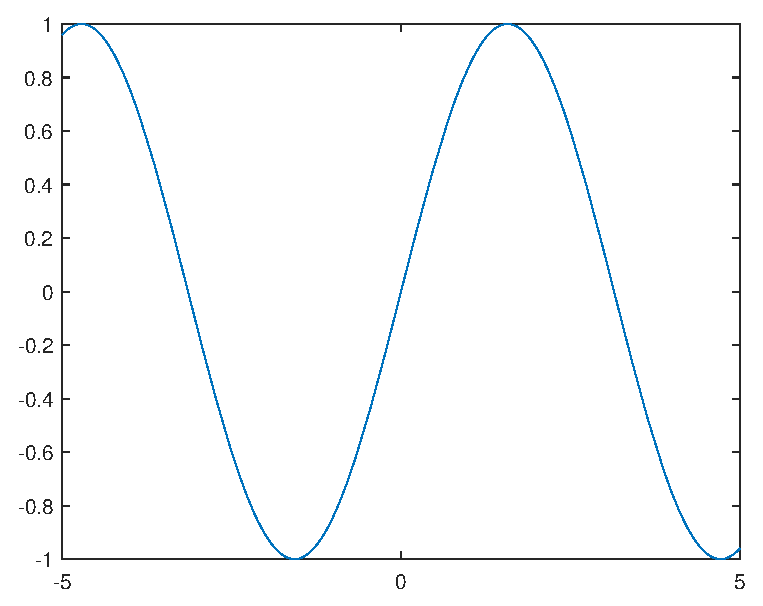
\includegraphics[width=0.48\textwidth]{image1}
\caption{Image of function $y=\sin(x)$}
\label{fig:sinx}
\end{figure}

Two pictures placed side by side, as shown in Figure~\ref{fig:image1} and Figure~\ref{fig:image2}.

\begin{figure}[!htp]
\begin{minipage}[h]{0.48\linewidth}
\centering
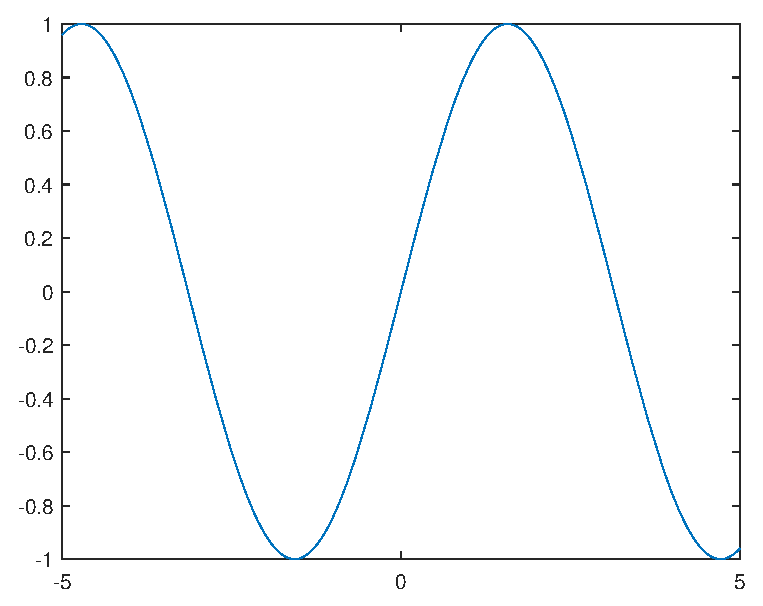
\includegraphics[width=0.9\textwidth]{image1}
\caption{Description of image 1}
\label{fig:image1}
\end{minipage}
\begin{minipage}[h]{0.48\linewidth}
\centering
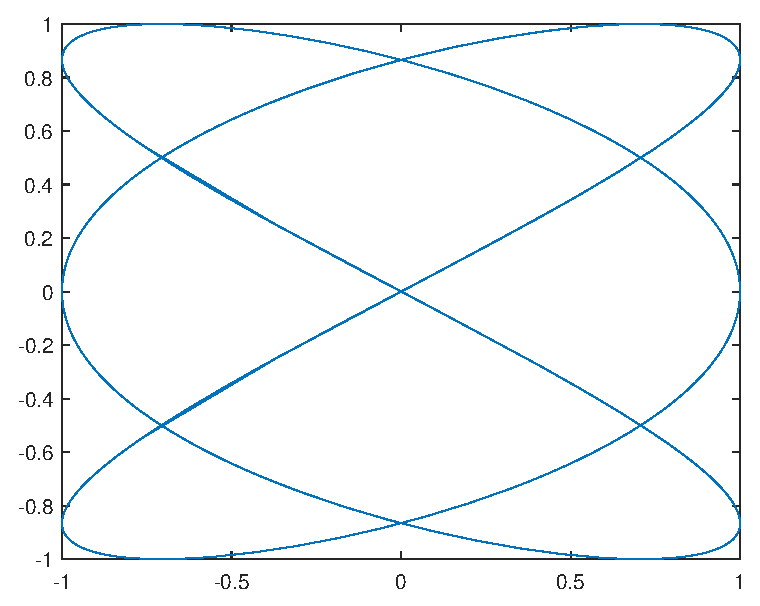
\includegraphics[width=0.9\textwidth]{image2}
\caption{Description of image 2}
\label{fig:image2}
\end{minipage}
\end{figure}


\clearpage
\section*{Code highlighting}

This is MATLAB code highlighting environment

% set code font
%basicstyle=\footnotesize\fontspec{Courier New}
%basicstyle=\footnotesize\fontspec{Consolas}

\begin{lstlisting}[style=matlab,title={MATLAB code}]
% Euler method for the ODE model
% u'(x)=x^2+x-u, x in [0,1]
% Initial condition: u(0)=0.
clear all;  clf
h=0.1;
x=0:h:1;
N=length(x)-1;
u(1)=0;
fun=@(t,u) t.^2+t-u;   % RHS
for n=1:N
    u(n+1)=u(n)+h.*fun(x(n),u(n));
end
ue=-exp(-x)+x.^2-x+1;  % exact solution
plot(x,ue,'b-',x,u,'r+','LineWidth',1)
legend('Exact','Numerical','location','North')
xlabel('x'), ylabel('u')
\end{lstlisting}

This is Python code highlighting environment

\begin{lstlisting}[style=python,title={Python code}]
#PythonDraw.py
import turtle as t
t.setup(650, 350, 200, 200)
t.penup()
t.fd(-250)
t.pendown()
t.pensize(25)
t.pencolor("purple color")
t.seth(-40)
for i in range(4):
    t.circle(40, 80)
    t.circle(-40, 80)
t.circle(40, 80/2)
t.fd(40)
t.circle(16, 180)
t.fd(40 * 2/3)
t.done()
\end{lstlisting}

%-------------------------%

\clearpage
\begin{thebibliography}{99}
\bibitem{Tadmor2012} E.~Tadmor. A review of numerical methods for nonlinear partial differential equations. Bull. Amer. Math. Soc., 2012, 49(4): 507-554.

\bibitem{Adams2003} R.~A.~ Adams, Fournier~J~J~F. Sobolev spaces. Elsevier, 2003.

\bibitem{TreWei2014} L.~N.~Trefethen, J.~A.~C.~Weideman. The exponentially convergent trapezoidal rule. SIAM Rev., 2014, 56(3): 385-458.

\bibitem{Shen1994} J.~Shen. Efficient spectral-Galerkin method I. Direct solvers of second- and fourth-order equations using Legendre polynomials. SIAM J. Sci. Comput., 1994, 15(6): 1489-1505.

\end{thebibliography}


\end{document}


